\capitulo{3}{Conceptos teóricos}

En este proyecto, el enfoque principal se centra en las redes convolucionales, tanto en el preprocesado llevado, como la creación a través de transferencia de aprendizaje. Además, hay que tener en cuenta que se debe crear una aplicación Android, donde estas redes estén incluidas.

\section{Conceptos de Redes Neuronales}

    En esta sección, se van a ver los conceptos más importantes de las redes neuronales convolucionales en el contexto de la inteligencia artificial.

    La inteligencia artificial es una rama de la ciencia de la computación que trata de imitar la inteligencia humana para realizar tareas, buscando simular la capacidad de aprendizaje y razonamiento que tienen los seres humanos, entre otras cosas. Algunos de los objetivos de la inteligencia artificial son: representación de conocimientos, aprendizaje automático, procesamiento del lenguaje natural, inteligencia social e inteligencia general~\cite{definicion_artificial_intelligence}.

    El aprendizaje automático, o \textit{machine learning}, es una rama de la inteligencia artificial, cuyo objetivo es que las máquinas aprendan por sí mismas a partir de los datos proporcionados. Se considera aprendizaje a la adquisición de conocimientos a través del estudio, la  experiencia o de ser enseñado; como esta definición no es útil para las máquinas, se define nombrando rendimiento en vez de conocimiento, así, se considera que el objetivo del aprendizaje es mejorar el rendimiento en futuras acciones~\cite{machine-learning}.
    El aprendizaje automático se apoya en clasificadores para generar un modelo. Entre los más comunes se encuentran: los árboles de decisión, las reglas de asociación, los algoritmos genéticos, las máquinas de soporte vectorial, \textit{clustering}, las redes bayesianas y las redes neuronales artificiales.
    Según la naturaleza del aprendizaje automático, se puede considerar uno de estos tipos: aprendizaje supervisado, aprendizaje no supervisado, aprendizaje semisupervisado y aprendizaje por refuerzo.
    
    El aprendizaje supervisado es un tipo de aprendizaje automático, en este se dispone de un conjunto de datos junto con el resultado que se espera obtener. Durante el entrenamiento, el modelo aprende a reconocer patrones y relaciones entre los datos de entrada y sus respectivas etiquetas, si el modelo está proporcionando resultados incorrectos, se pueden corregir de forma que se obtengan mejores resultados. Con el modelo ya entrenado, se pueden obtener predicciones de datos no vistos. Un problema que surge es el \textit{overfitting}, el cual hace que el modelo aprenda los datos, dando los resultados correspondientes para cada instancia.

    El aprendizaje supervisado se ha beneficiado enormemente de los avances en las redes neuronales artificiales (RNN). Estas redes son modelos computacionales  con al menos una capa oculta~\cite{definicion_neural_network}, la cual consiste en una o más neuronas donde cada una calcula la suma de los valores de entrada, multiplicados por su peso correspondiente~\cite{definicion_hidden_layer}. En la figura~\ref{fig:funcionamientoRedNeuronal}, se puede observar una red neuronal, donde cada círculo representa una neurona artificial, y las flechas la conexión entre las distintas neuronas.

    \begin{figure}[!ht]
         \centering
         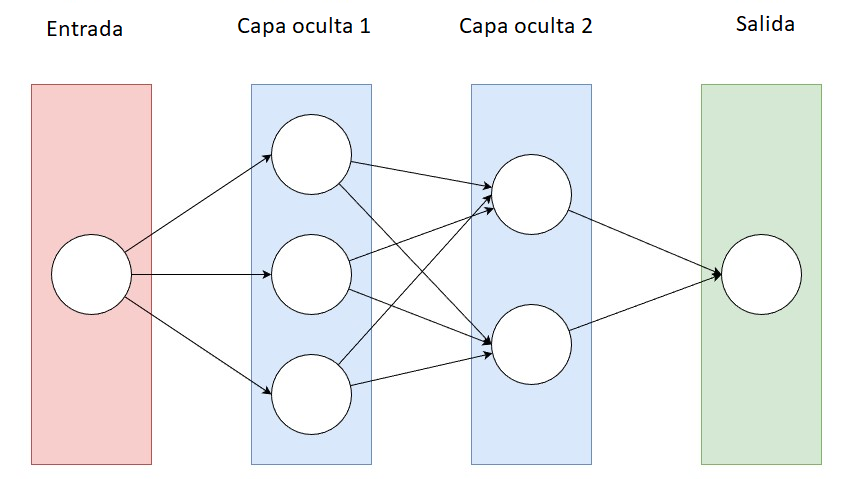
\includegraphics[width=0.9\textwidth]{img/RedNeuronal.png}
         \caption{Funcionamiento de una red neuronal}
         \label{fig:funcionamientoRedNeuronal}
    \end{figure}
    El valor calculado se utiliza en una función de activación, que produce el valor de salida\cite{definicion_activation_function}. Entre las funciones de activación destacan las visibles en \ref{fig:funciones_de_activacion}.
    \begin{itemize}
        \item La función RELU (verde), la cual indica el máximo entre 0 y el valor calculado~\ref{fig:funcionRELU}.
        \item La función lineal(rosa), la cual devuelve el mismo valor calculado~\ref{fig:funcionLineal}.
        \item La función sigmoidea(cían), la cual devuelve un valor entre 0 y 1 según lo alejado que este del 0~\ref{fig:funcionSigmoidal}.
        \item La función escalón(morada), devuelve o 0 o 1 dependiendo del signo del valor calculado~\ref{fig:funcionEscalon}.
    \end{itemize}
    
 \begin{figure}[!ht]
        \centering
        \begin{subfigure}{0.45\textwidth}
            \centering
            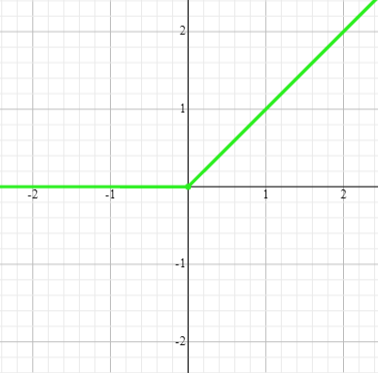
\includegraphics[width=\textwidth]{img/RELU.png}
            \caption{RELU}
            \label{fig:funcionRELU}
        \end{subfigure}
        \begin{subfigure}{0.45\textwidth}
            \centering
            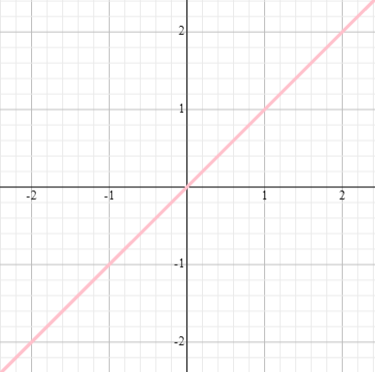
\includegraphics[width=\textwidth]{img/lineal.png}
            \caption{Lineal}
            \label{fig:funcionLineal}
        \end{subfigure}

        \vspace{1em}

        \begin{subfigure}{0.45\textwidth}
            \centering
            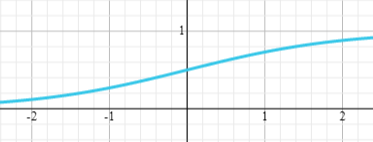
\includegraphics[width=\textwidth]{img/Sigmoidal.png}
            \caption{Sigmoidea}
            \label{fig:funcionSigmoidal}
        \end{subfigure}
        \begin{subfigure}{0.45\textwidth}
            \centering
            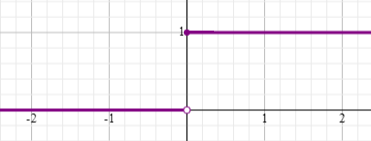
\includegraphics[width=\textwidth]{img/escalon.png}
            \caption{Escalón}
            \label{fig:funcionEscalon}
        \end{subfigure}

        \caption{Funciones de activación}
        \label{fig:funciones_de_activacion}
    \end{figure}

    Para hacer más visual una red neuronal, se hará un ejemplo, suponemos una asignatura, donde un alumno realiza 2 exámenes, 2 trabajos prácticos y 1 trabajo final. La nota final de la asignatura se corresponde a un 50\% de los exámenes, donde el primer examen vale un 40\% y el segundo un 60\%, un 30\% a los trabajos prácticos, donde ambos tienen el mismo porcentaje, y el trabajo final que vale un 20\%. 
    
    El profesor de la asignatura quiere saber si un alumno ha aprobado o suspendido, con las siguientes notas: un 8 en el primer examen, un 1 en el segundo, en ambos trabajos prácticos un 5 y en el trabajo final un 6.

    En la figura  \ref{fig:ejemploRedNeuronal} se observa la ejemplificación de la red, donde la capa roja se corresponde a la capa de entrada, la capa azul con la capa oculta de la red, y la capa verde con la capa de salida. En este caso, en la capa oculta se ha usado una función de activación RELU, obteniendo los valores de dentro de los círculos, y en la capa de salida, se utiliza una función escalón, con un bias de -5, en este caso, el alumno habría obtenido una nota de 4,6, como la suma de -5 + 4,6 es menor que 0, lo que significaría que el alumno ha suspendido.
    
    \begin{figure}[!ht]
         \centering
         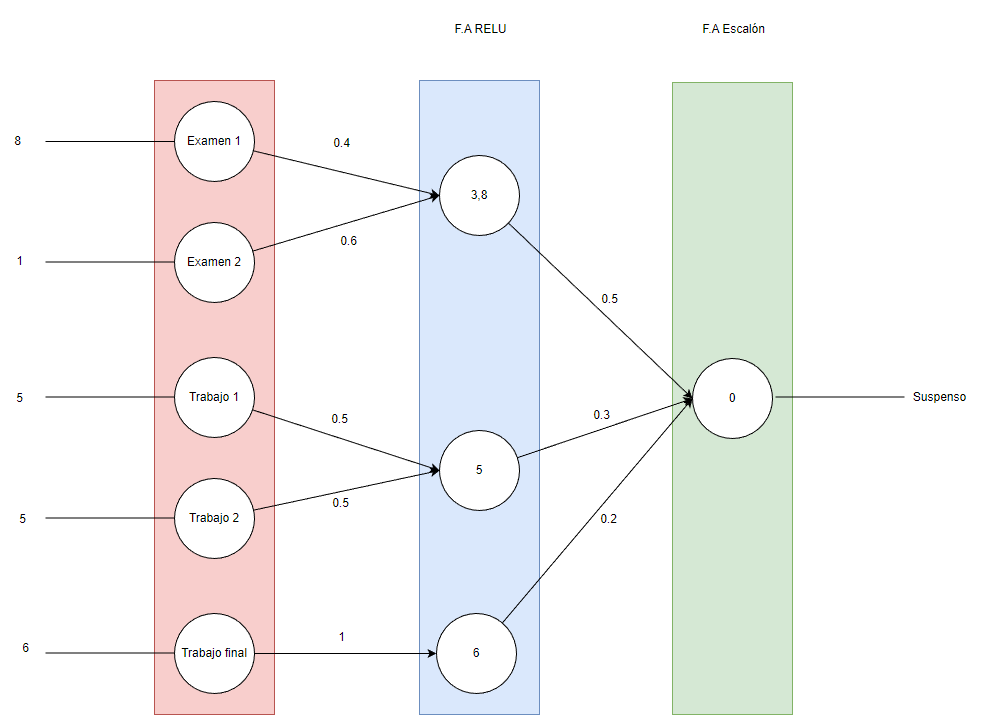
\includegraphics[width=0.9\textwidth]{img/Ejemplo Red Neuronal.png}
         \caption{Ejemplo de una red neuronal}
         \label{fig:ejemploRedNeuronal}
    \end{figure}
    
     Dentro de las redes neuronales, se encuentran las redes neuronales convolucionales (CNN), estas redes son las que poseen al menos una capa convolucional, consistiendo en la combinación de capas convolucionales, capas de agrupación y capas densas~\cite{definicion_CNN}.

     Una capa convolucional es un conjunto de neuronas artificiales que realizan varias series de operaciones convolucionales, actuando cada una sobre una submatriz de la matriz de entrada~\cite{definicionConvolucional_layer}.
     
     Una operación convolucional es aquella que a partir de una submatriz de la matriz de entrada (donde a veces es necesario realizar un filtrado para ponderar los datos) se calcula la suma de los valores de esta submatriz asignando el resultado a la matriz de salida~\cite{definicionConvolutional_Operation}.
     
     La capa de agrupación es una capa de una red neuronal que reduce el tamaño de la matriz de entrada, mediante operaciones como el máximo o la media de los valores de una submatriz~\cite{definicion_pooling}.

     La capa densa también llamada capa totalmente conectada, es una capa oculta, donde cada nodo está conectado a todos los nodos de la siguiente capa oculta~\cite{definicion_fully_connected_layer}.
     
    Una red neuronal residual es aquella que permite el salto de capas intermedias. Estas conexiones permiten que la red aprenda las características residuales, es decir, las diferencias entre las entradas y las salidas esperadas.  Para ello, se crea un bloque residual, que en lugar de transmitir la salida de una capa directamente a la siguiente, se introduce una conexión residual que suma la salida de una capa a la entrada de otra capa posterior como se puede ver en \ref{fig:residual-block}.

\begin{figure}[!ht]
         \centering
         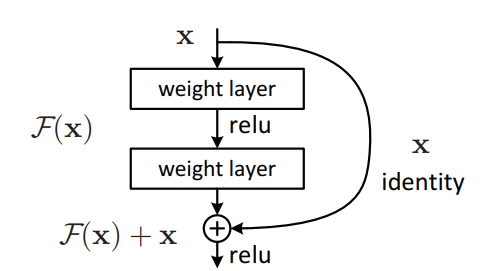
\includegraphics[width=0.6\textwidth]{img/residual-block.png}
         \caption{Bloque residual. Imagen extraída de~\cite{DBLP:journals/corr/HeZRS15}.}
         \label{fig:residual-block}
\end{figure}
\section{Preprocesado}
En el proyecto, se han realizado varios preprocesados, puesto que hay varias redes neuronales convolucionales.

\subsection{Red neuronal convolucional VGG16, para la calidad de la imagen}

En una red neuronal convolucional VGG16, el preprocesado necesario es que la imagen en vez de estar en formato RGB (Rojo, verde y azul), está en un formato BGR(Azul, verde y rojo), donde la diferencia entre estos formatos es el orden en el que se encuentran los colores, y en el preprocesado, también es necesario que los valores finales estén centralizados en 0. Además de este cambio, la imagen debe tener de 224 x 224 píxeles, redimensionando las imágenes que se introduzcan a la red.
\cite{tensorflowVGG16}
Para realizar este preprocesado en Python, se puede llamar a la función \textit{tf.keras.applications.vgg16.preprocess\_input}, para la aplicación de Android Studio, se ha implementado este preprocesamiento.
La estructura de la red convolucional VGG16, se puede observar en la figura \ref{fig:VGG-16-struct}, donde hay 13 capas convolucionales, y  4 de agrupación. 
\begin{figure}[!ht]
         \centering
         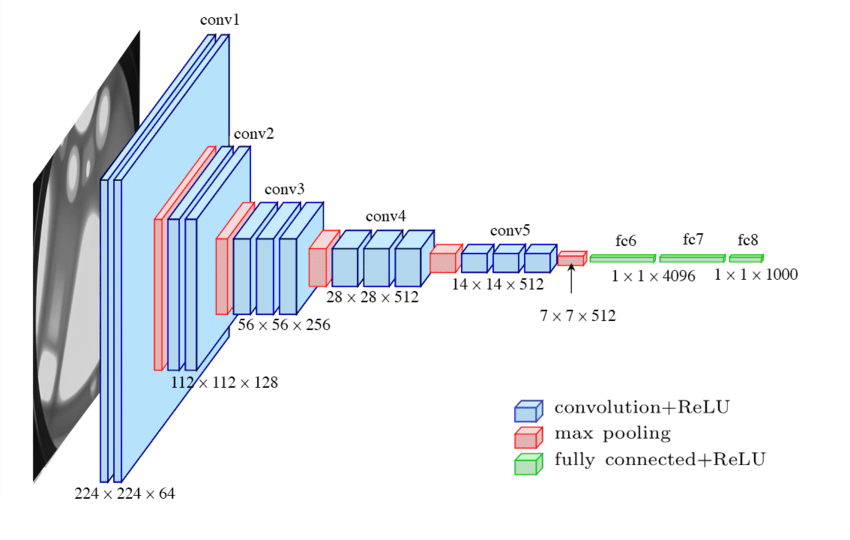
\includegraphics[width=0.9\textwidth]{img/VGG-16-network-architecture.png}
         \caption{Estructura básica de la red convolucional VGG16. Imagen extraída de~\cite{vgg16-structure}}
         \label{fig:VGG-16-struct}
\end{figure}


\subsection{Red neuronal convolucional ResNet50V2, para la detección de retinopatía}

La red ResNet50V2 es una red neuronal residual que, como se ha comentado anteriormente, permite saltarse capas, como se puede ver en la figura~\ref{fig:residual-block}.

En la red neuronal convolucional ResNet50V2, el procesamiento es distinto al de VGG16, la gama de color es RGB, también se tiene que normalizar los datos, pero en este caso, el intervalo es [-1,1]~\cite{tensorflowResNet50V2}.

Esta red neuronal ya estaba entrenada, por tanto, no se tuvo que hacer ningún preprocesado en Python; pero al implementar la red en Android Studio, al igual que en la red VGG16, se debía realizar el preprocesamiento a mano.

Donde la formula para cambiar este valor vendría dada por: 
\begin{center}
    $ColorPreprocesado = (ColorSinPreprocesar - 0)/ 255.0 * 2 - 1$
    \begin{itemize}
        \item Donde 0 representa el valor mínimo que puede tomar el color en concreto.
        \item Donde 255 representa el valor máximo que puede tomar el color en concreto.
        \item Y donde $ * 2 - 1 $ es la operación para normalizar el valor en formato [-1, 1]
    \end{itemize}
\end{center}

La estructura de la red convolucional ResNet50V2, se puede observar en la figura~\ref{fig:ResNet50v2-struct}, en esta red neuronal convolucional,  hay 50 capas repartidas entre 5 bloques. El primer bloque no es convolucional, pero los otros 4 sí que contienen capas convolucionales de tamaños variados, incluyendo convoluciones de 1x1, 3x3 y 1x1.
\begin{figure}[!ht]
         \centering
         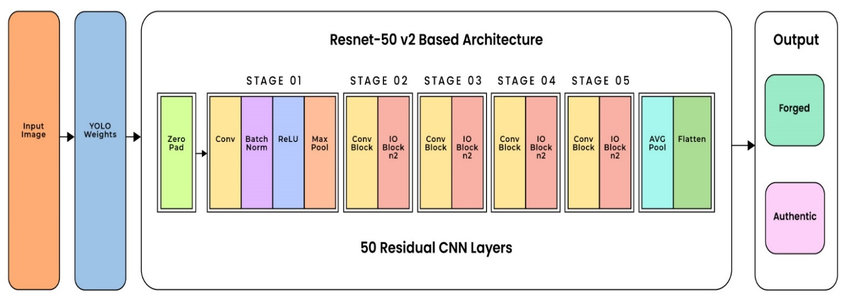
\includegraphics[width=0.9\textwidth]{img/ResNet50v2-architecture.jpg}
         \caption{Estructura básica de la red convolucional ResNet50v2. Imagen extraída de~\cite{ResNet50v2-architecture}}
         \label{fig:ResNet50v2-struct}
\end{figure}

\section{Transfer learning}

El aprendizaje transferido o ``Transfer learning'' es una técnica del \textit{Machine learning}, la cual consiste en reutilizar el conocimiento ya aprendido de un modelo, en otra actividad que tenga un objetivo similar. 

En el ámbito que nos concierne, se ha utilizado el modelo VGG-16 que ha sido entrenado con el dataset de ImageNet ``Large Scale Visual Recognition Challenge 2014 (ILSVRC2014) ''. El objetivo de este modelo es clasificar imágenes entre 1.000 categorías distintas, aprendiendo las características visuales de cada una. 

Para transferir el modelo, es necesario congelar las capas, para que no se entrenen. Con esto realizado, solo falta obtener el resultado, que puede ser binario o multiclase dependiendo del problema.

Además, se ha agregado una capa de agrupación para hacer uso de las capas densas. La primera capa densa consta de 64 neuronas con una función de activación RELU. Por otro lado, la segunda capa densa actúa como la capa de salida, y su propósito es evaluar la calidad de la imagen.

El código de creación del modelo sería el siguiente:

\lstset{
  language=Python,
  basicstyle=\small\ttfamily,
  keywordstyle=\color{blue},
  commentstyle=\color{green!60!black},
  stringstyle=\color{red},
  showstringspaces=false,
  breaklines=true,
  breakatwhitespace=true,
  tabsize=4,
  numbers=none,
  numberstyle=\tiny,
  frame=single,
  framexleftmargin=5mm,
  xleftmargin=5mm
}
\begin{lstlisting}
vgg16 = VGG16(include_top=False, weights='imagenet', input_shape=(224, 224, 3))
for layer in vgg16.layers:
    layer.trainable = False
model = Sequential()
model.add(vgg16)
model.add(tensorflow.keras.layers.Flatten())
model.add(tensorflow.keras.layers.Dense(64, activation='relu'))
model.add(tensorflow.keras.layers.Dense(num_classes, activation='sigmoid'))

\end{lstlisting}

\section{Formato de la red neuronal}

El formato de las redes neuronales convolucionales suele venir dado en formato ``.h5'' o keras, para facilitar la implementación en Android Studio, se ha tenido que transformar este archivo en formato TensorFlow Lite, el cual requiere menos recursos, permitiendo su integración en dispositivos móviles.

Para realizar esta conversión, se ha utilizado un fichero Python, el cual se ha buscado en la documentación de TensorFlow Lite, y posteriormente, guardar el fichero~\cite{tensorflowliteConverter}.

En el siguiente código, se puede observar el convertidor, donde file es el directorio donde se encontraría el archivo keras, nombre es el nombre de este fichero, y fileSalida es el directorio de salida.
\lstset{
  language=Python,
  basicstyle=\ttfamily,
  keywordstyle=\color{blue},
  commentstyle=\color{green!60!black},
  stringstyle=\color{red},
  showstringspaces=false,
  breaklines=true,
  breakatwhitespace=true,
  tabsize=4,
  numbers=none,
  numberstyle=\tiny,
  frame=single,
  framexleftmargin=5mm,
  xleftmargin=5mm
}
\begin{lstlisting}
model = tf.keras.models.load_model(file+nombre+'.h5')
converter = tf.lite.TFLiteConverter.from_keras_model(model)
tflite_model= converter.convert()
nombreSalida = "calidad.tflite"
with open(fileSalida+nombre+'.tflite', 'wb') as f:
    f.write(tflite_model)

\end{lstlisting}
\section{Desbalanceo de los datos}

Para la minería de datos, el problema de que los datos estén desbalanceados causa que los modelos entrenados suelan producir resultados indebidos.

Un ejemplo del desbalanceo de datos, podría ser un modelo que entrena los números diciendo si son primos o no. En este caso, si se calcula el modelo por porcentaje de aciertos, en caso de devolver siempre que el número introducido no es primo, esta medida tiende a ser del 100\%.
Por este motivo, se suelen usar otras métricas u otras formas de entrenar al modelo, para que se evite la disparidad de los datos.

La forma de solucionar este problema en este trabajo ha sido usando otras medidas como podrían ser precisión, recall y F1Score.
En la figura \ref{fig:matrizDeConfusion} se puede observar la matriz de confusión de positivos y negativos. A partir de la cual, se explicaran las medidas.
\begin{figure}[!ht]
         \centering
         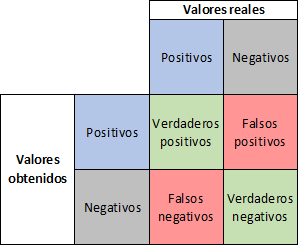
\includegraphics[width=0.6\textwidth]{img/Matriz de confusion.png}
          \caption{Matriz de confusión}
         \label{fig:matrizDeConfusion}
\end{figure}

La precisión es el numero de Verdaderos positivos entre la suma de verdaderos positivos y falsos positivos.
\begin{center}
    $Precision = \dfrac{Verdaderos Positivos} {Verdaderos Positivos + Falsos Positivos} $
\end{center}

Por otro lado, el recall, es el número de verdaderos positivos entre la suma de los verdaderos positivos y los falsos negativos.
\begin{center}
    $Recall = \dfrac{Verdaderos Positivos} {Verdaderos Positivos + Falsos Negativos} $
\end{center}

F1 Score es una medida obtenida de las dos anteriores, siendo la media armónica de estas.
\begin{center}
    $F_1 = 2 \dfrac{Precision * Recall} {Precision + Recall} $
\end{center}

En el caso concreto, una imagen puede ser APTA o NO\_APTA, encontrándose el desbalanceo de imágenes de 455 APTA y 103 NO\_APTA. De esta forma, se ha considerado en la matriz \ref{fig:matrizDeConfusion}, como ``Positivos'' a la clase NO\_APTA y como ``Negativos'' a la clase APTA.

La otra opción que no se ha utilizado, pero es importante destacarla, es el uso de oversampling o undersampling. Estas técnicas buscan igualar número de entidades en el conjunto de datos según la clase. 

Mientras oversampling, busca añadir datos a partir del conjunto de datos, duplicando o modificando los datos entre distintas instancias. Esta opción no se ha ni planteado, puesto que si se duplican las imágenes NO\_APTA, lo que va a producir es sobreajuste del modelo; y suponiendo que los datos nuevos fuesen modificaciones de combinaciones de imágenes  NO\_APTA, se estaría introduciendo ruido, puesto que crearía imágenes no reales.

El undersampling al contrario que el oversampling, elimina datos del grupo mayoritario, hasta que hay un número similar de instancias, las instancias eliminadas se pueden utilizar para validación o para test. Al implementar este método, se pueden eliminar inicialmente instancias que clasifican muy bien el modelo, haciendo que dependa el código de la inicialización del conjunto de entrenamiento y del conjunto de test.

\section{Guías de diseño Android}

Para realizar la aplicación se siguió la guía de diseño de Google Material3.

En los botones, se recomienda la forma circular en las esquinas, de forma que sea más visible para los ojos. En la figura \ref{fig:EsquinasRedondeadas} se puede ver la comparación entre las esquinas con pico y redondeadas, en esta explica que las formas con esquinas hacen que el enfoque esté fuera del rectángulo, mientras que en las redondeadas consigue que el enfoque esté dentro.
        \begin{figure}[!ht]
                 \centering
                 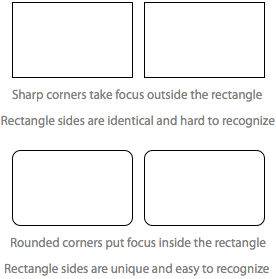
\includegraphics[width=0.45\textwidth]{img/rounded-corners.png}
                  \caption{Diferencias esquinas. Imagen obtenida de~\cite{rounded-corners-uxmovement}}
                 \label{fig:EsquinasRedondeadas}
        \end{figure}

Para los colores de la aplicación, como es una aplicación orientada en el bienestar y salud de las personas, estos colores tenían que ser claros con tonos verdes y azules, colores usados también en el diseño del logo de la aplicación, por otro lado, hay personas que prefieren un fondo oscuro a uno claro, por lo que se incluyo la opción de modo oscuro en la aplicación.

La gamma de color usada fue: en modo claro, gris claro para el fondo \#E0E0E0 y los botones azules claros \#90CAF9,  y para el modo oscuro, gris oscuro para el fondo \#353740 y los botones verdes claros.
Para el color del texto, varía entre blanco y negro según el fondo. Buscando en todo momento contraste  entre los objetos y el fondo de la aplicación.

Durante la ejecución de la aplicación, es preferible que los distintos objetos estén deshabilitados, a invisibles, de esta forma, el usuario entiende que si interactúa con la aplicación, ese objeto se habilitará. Como es el caso de la realización de la foto, que hasta que el usuario no haya seleccionado una imagen no puede pasar a la siguiente pantalla. Esto es contraproducente en algunos casos, puesto que los mensajes de error es mejor mostrarlos solo cuando el error ocurre; como es el caso de iniciar sesión incorrectamente o el caso de que la calidad de la imagen sea baja.